\documentclass[1p]{elsarticle_modified}
%\bibliographystyle{elsarticle-num}

%\usepackage[colorlinks]{hyperref}
%\usepackage{abbrmath_seonhwa} %\Abb, \Ascr, \Acal ,\Abf, \Afrak
\usepackage{amsfonts}
\usepackage{amssymb}
\usepackage{amsmath}
\usepackage{amsthm}
\usepackage{scalefnt}
\usepackage{amsbsy}
\usepackage{kotex}
\usepackage{caption}
\usepackage{subfig}
\usepackage{color}
\usepackage{graphicx}
\usepackage{xcolor} %% white, black, red, green, blue, cyan, magenta, yellow
\usepackage{float}
\usepackage{setspace}
\usepackage{hyperref}

\usepackage{tikz}
\usetikzlibrary{arrows}

\usepackage{multirow}
\usepackage{array} % fixed length table
\usepackage{hhline}

%%%%%%%%%%%%%%%%%%%%%
\makeatletter
\renewcommand*\env@matrix[1][\arraystretch]{%
	\edef\arraystretch{#1}%
	\hskip -\arraycolsep
	\let\@ifnextchar\new@ifnextchar
	\array{*\c@MaxMatrixCols c}}
\makeatother %https://tex.stackexchange.com/questions/14071/how-can-i-increase-the-line-spacing-in-a-matrix
%%%%%%%%%%%%%%%

\usepackage[normalem]{ulem}

\newcommand{\msout}[1]{\ifmmode\text{\sout{\ensuremath{#1}}}\else\sout{#1}\fi}
%SOURCE: \msout is \stkout macro in https://tex.stackexchange.com/questions/20609/strikeout-in-math-mode

\newcommand{\cancel}[1]{
	\ifmmode
	{\color{red}\msout{#1}}
	\else
	{\color{red}\sout{#1}}
	\fi
}

\newcommand{\add}[1]{
	{\color{blue}\uwave{#1}}
}

\newcommand{\replace}[2]{
	\ifmmode
	{\color{red}\msout{#1}}{\color{blue}\uwave{#2}}
	\else
	{\color{red}\sout{#1}}{\color{blue}\uwave{#2}}
	\fi
}

\newcommand{\Sol}{\mathcal{S}} %segment
\newcommand{\D}{D} %diagram
\newcommand{\A}{\mathcal{A}} %arc


%%%%%%%%%%%%%%%%%%%%%%%%%%%%%5 test

\def\sl{\operatorname{\textup{SL}}(2,\Cbb)}
\def\psl{\operatorname{\textup{PSL}}(2,\Cbb)}
\def\quan{\mkern 1mu \triangleright \mkern 1mu}

\theoremstyle{definition}
\newtheorem{thm}{Theorem}[section]
\newtheorem{prop}[thm]{Proposition}
\newtheorem{lem}[thm]{Lemma}
\newtheorem{ques}[thm]{Question}
\newtheorem{cor}[thm]{Corollary}
\newtheorem{defn}[thm]{Definition}
\newtheorem{exam}[thm]{Example}
\newtheorem{rmk}[thm]{Remark}
\newtheorem{alg}[thm]{Algorithm}

\newcommand{\I}{\sqrt{-1}}
\begin{document}

%\begin{frontmatter}
%
%\title{Boundary parabolic representations of knots up to 8 crossings}
%
%%% Group authors per affiliation:
%\author{Yunhi Cho} 
%\address{Department of Mathematics, University of Seoul, Seoul, Korea}
%\ead{yhcho@uos.ac.kr}
%
%
%\author{Seonhwa Kim} %\fnref{s_kim}}
%\address{Center for Geometry and Physics, Institute for Basic Science, Pohang, 37673, Korea}
%\ead{ryeona17@ibs.re.kr}
%
%\author{Hyuk Kim}
%\address{Department of Mathematical Sciences, Seoul National University, Seoul 08826, Korea}
%\ead{hyukkim@snu.ac.kr}
%
%\author{Seokbeom Yoon}
%\address{Department of Mathematical Sciences, Seoul National University, Seoul, 08826,  Korea}
%\ead{sbyoon15@snu.ac.kr}
%
%\begin{abstract}
%We find all boundary parabolic representation of knots up to 8 crossings.
%
%\end{abstract}
%\begin{keyword}
%    \MSC[2010] 57M25 
%\end{keyword}
%
%\end{frontmatter}

%\linenumbers
%\tableofcontents
%
\newcommand\colored[1]{\textcolor{white}{\rule[-0.35ex]{0.8em}{1.4ex}}\kern-0.8em\color{red} #1}%
%\newcommand\colored[1]{\textcolor{white}{ #1}\kern-2.17ex	\textcolor{white}{ #1}\kern-1.81ex	\textcolor{white}{ #1}\kern-2.15ex\color{red}#1	}

{\Large $\underline{10_{91}~(K10a_{106})}$}

\setlength{\tabcolsep}{10pt}
\renewcommand{\arraystretch}{1.6}
\vspace{1cm}\begin{tabular}{m{100pt}>{\centering\arraybackslash}m{274pt}}
\multirow{5}{120pt}{
	\centering
	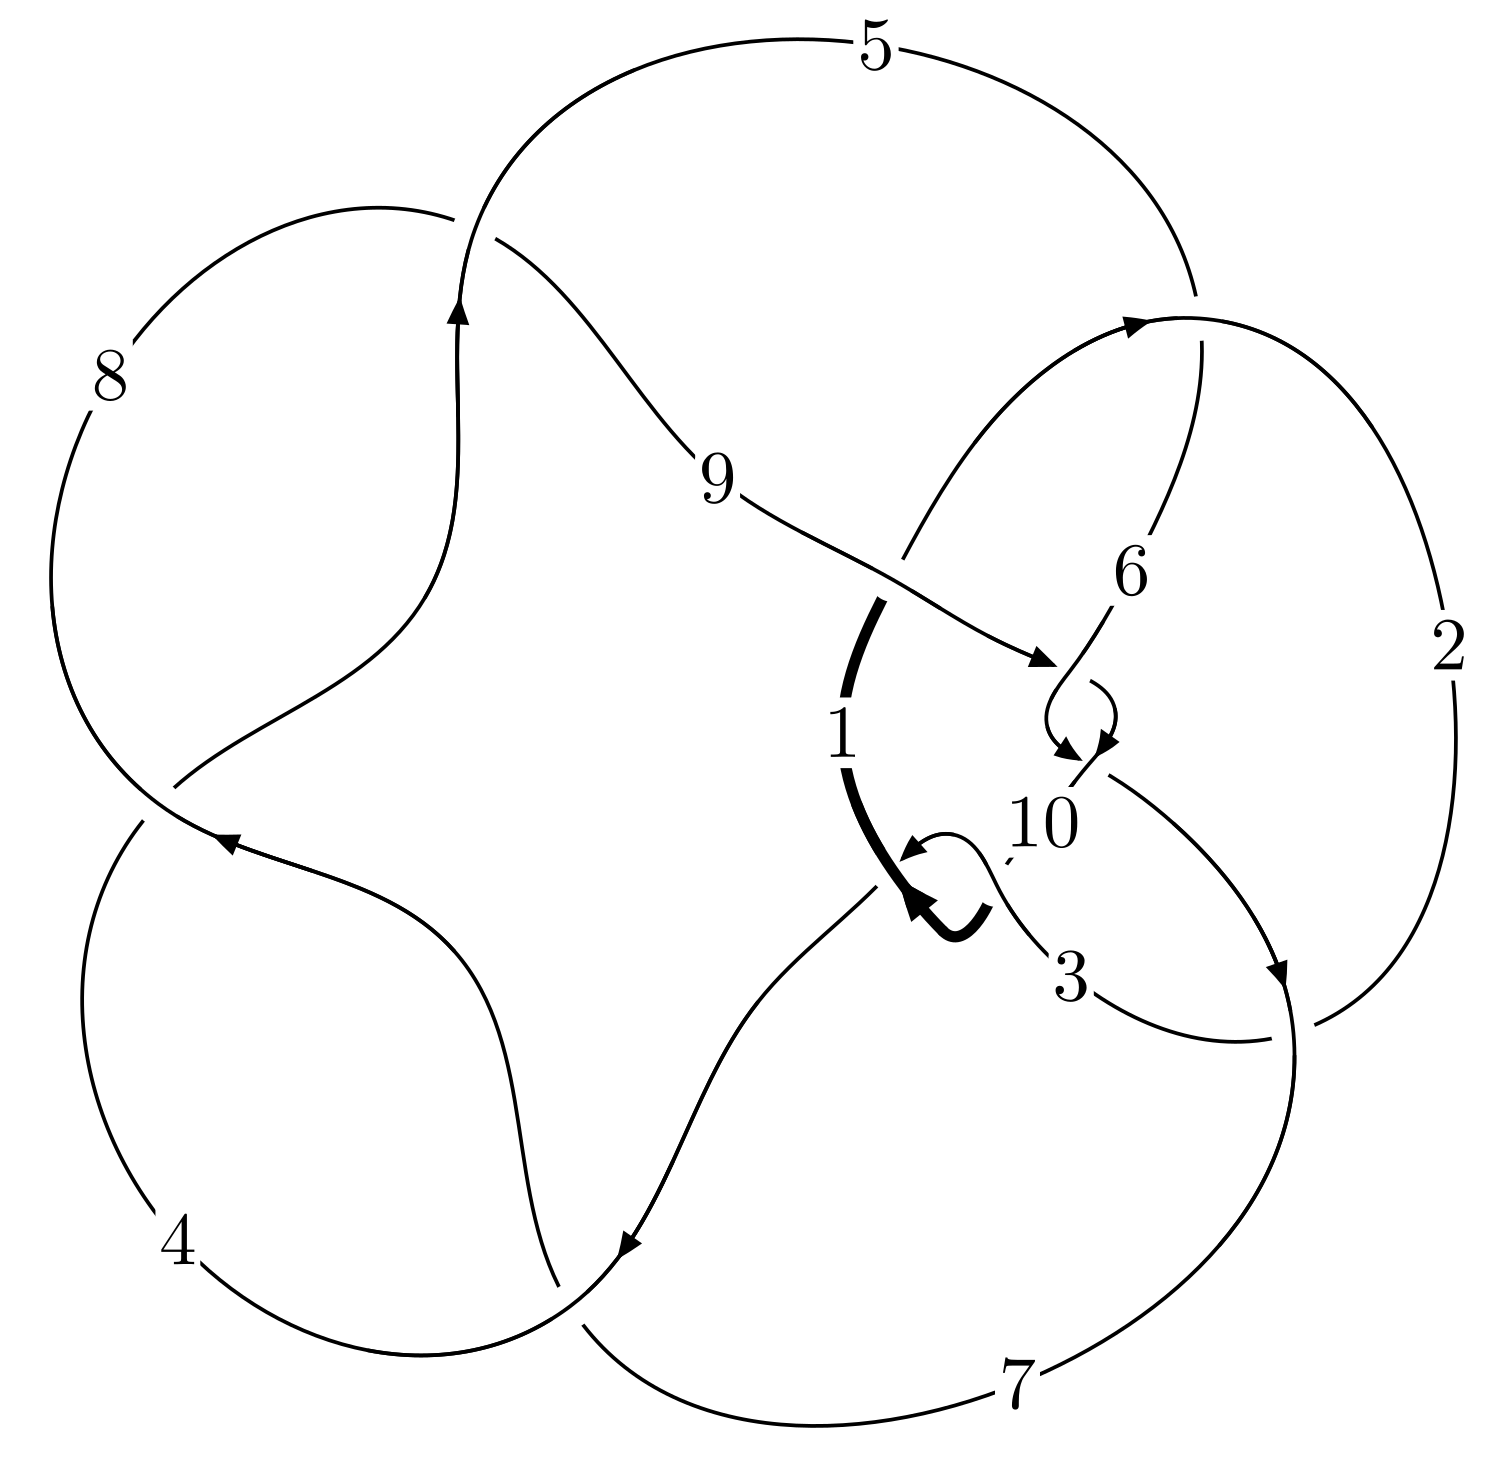
\includegraphics[width=112pt]{../../../GIT/diagram.site/Diagrams/png/175_10_91.png}\\
\ \ \ A knot diagram\footnotemark}&
\allowdisplaybreaks
\textbf{Linearized knot diagam} \\
\cline{2-2}
 &
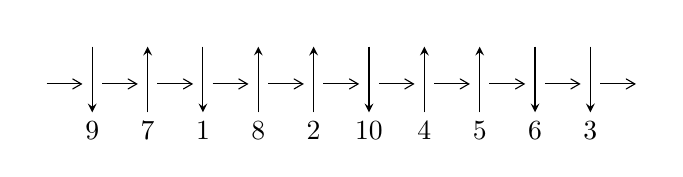
\begin{tikzpicture}[x=20pt, y=17pt]
	% nodes
	\node (C0) at (0, 0) {};
	\node (C1) at (1, 0) {};
	\node (C1U) at (1, +1) {};
	\node (C1D) at (1, -1) {9};

	\node (C2) at (2, 0) {};
	\node (C2U) at (2, +1) {};
	\node (C2D) at (2, -1) {7};

	\node (C3) at (3, 0) {};
	\node (C3U) at (3, +1) {};
	\node (C3D) at (3, -1) {1};

	\node (C4) at (4, 0) {};
	\node (C4U) at (4, +1) {};
	\node (C4D) at (4, -1) {8};

	\node (C5) at (5, 0) {};
	\node (C5U) at (5, +1) {};
	\node (C5D) at (5, -1) {2};

	\node (C6) at (6, 0) {};
	\node (C6U) at (6, +1) {};
	\node (C6D) at (6, -1) {10};

	\node (C7) at (7, 0) {};
	\node (C7U) at (7, +1) {};
	\node (C7D) at (7, -1) {4};

	\node (C8) at (8, 0) {};
	\node (C8U) at (8, +1) {};
	\node (C8D) at (8, -1) {5};

	\node (C9) at (9, 0) {};
	\node (C9U) at (9, +1) {};
	\node (C9D) at (9, -1) {6};

	\node (C10) at (10, 0) {};
	\node (C10U) at (10, +1) {};
	\node (C10D) at (10, -1) {3};
	\node (C11) at (11, 0) {};

	% arrows
	\draw[->,>={angle 60}]
	(C0) edge (C1) (C1) edge (C2) (C2) edge (C3) (C3) edge (C4) (C4) edge (C5) (C5) edge (C6) (C6) edge (C7) (C7) edge (C8) (C8) edge (C9) (C9) edge (C10) (C10) edge (C11) ;	\draw[->,>=stealth]
	(C1U) edge (C1D) (C2D) edge (C2U) (C3U) edge (C3D) (C4D) edge (C4U) (C5D) edge (C5U) (C6U) edge (C6D) (C7D) edge (C7U) (C8D) edge (C8U) (C9U) edge (C9D) (C10U) edge (C10D) ;
	\end{tikzpicture} \\
\hhline{~~} \\& 
\textbf{Solving Sequence} \\ \cline{2-2} 
 &
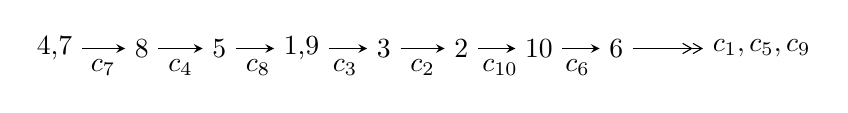
\begin{tikzpicture}[x=28pt, y=7pt]
	% node
	\node (A0) at (-1/8, 0) {4,7};
	\node (A1) at (1, 0) {8};
	\node (A2) at (2, 0) {5};
	\node (A3) at (49/16, 0) {1,9};
	\node (A4) at (33/8, 0) {3};
	\node (A5) at (41/8, 0) {2};
	\node (A6) at (49/8, 0) {10};
	\node (A7) at (57/8, 0) {6};
	\node (C1) at (1/2, -1) {$c_{7}$};
	\node (C2) at (3/2, -1) {$c_{4}$};
	\node (C3) at (5/2, -1) {$c_{8}$};
	\node (C4) at (29/8, -1) {$c_{3}$};
	\node (C5) at (37/8, -1) {$c_{2}$};
	\node (C6) at (45/8, -1) {$c_{10}$};
	\node (C7) at (53/8, -1) {$c_{6}$};
	\node (A8) at (9, 0) {$c_{1},c_{5},c_{9}$};

	% edge
	\draw[->,>=stealth]	
	(A0) edge (A1) (A1) edge (A2) (A2) edge (A3) (A3) edge (A4) (A4) edge (A5) (A5) edge (A6) (A6) edge (A7) ;
	\draw[->>,>={angle 60}]	
	(A7) edge (A8);
\end{tikzpicture} \\ 

\end{tabular} \\

\footnotetext{
The image of knot diagram is generated by the software ``\textbf{Draw programme}" developed by Andrew Bartholomew(\url{http://www.layer8.co.uk/maths/draw/index.htm\#Running-draw}), where we modified some parts for our purpose(\url{https://github.com/CATsTAILs/LinksPainter}).
}\phantom \\ \newline 
\centering \textbf{Ideals for irreducible components\footnotemark of $X_{\text{par}}$} 
 
\begin{align*}
I^u_{1}&=\langle 
2.01404\times10^{18} u^{35}-4.78501\times10^{18} u^{34}+\cdots+1.28887\times10^{18} b-6.30993\times10^{17},\\
\phantom{I^u_{1}}&\phantom{= \langle  }1.95116\times10^{19} u^{35}-6.14010\times10^{19} u^{34}+\cdots+1.41776\times10^{19} a+2.81287\times10^{18},\;u^{36}-3 u^{35}+\cdots+3 u^2+1\rangle \\
\\
\end{align*}
\raggedright * 1 irreducible components of $\dim_{\mathbb{C}}=0$, with total 36 representations.\\
\footnotetext{All coefficients of polynomials are rational numbers. But the coefficients are sometimes approximated in decimal forms when there is not enough margin.}
\newpage
\renewcommand{\arraystretch}{1}
\centering \section*{I. $I^u_{1}= \langle 2.01\times10^{18} u^{35}-4.79\times10^{18} u^{34}+\cdots+1.29\times10^{18} b-6.31\times10^{17},\;1.95\times10^{19} u^{35}-6.14\times10^{19} u^{34}+\cdots+1.42\times10^{19} a+2.81\times10^{18},\;u^{36}-3 u^{35}+\cdots+3 u^2+1 \rangle$}
\flushleft \textbf{(i) Arc colorings}\\
\begin{tabular}{m{7pt} m{180pt} m{7pt} m{180pt} }
\flushright $a_{4}=$&$\begin{pmatrix}0\\u\end{pmatrix}$ \\
\flushright $a_{7}=$&$\begin{pmatrix}1\\0\end{pmatrix}$ \\
\flushright $a_{8}=$&$\begin{pmatrix}1\\- u^2\end{pmatrix}$ \\
\flushright $a_{5}=$&$\begin{pmatrix}u\\- u^3+u\end{pmatrix}$ \\
\flushright $a_{1}=$&$\begin{pmatrix}-1.37623 u^{35}+4.33085 u^{34}+\cdots-3.87762 u-0.198403\\-1.56264 u^{35}+3.71256 u^{34}+\cdots-0.845601 u+0.489570\end{pmatrix}$ \\
\flushright $a_{9}=$&$\begin{pmatrix}- u^2+1\\u^4-2 u^2\end{pmatrix}$ \\
\flushright $a_{3}=$&$\begin{pmatrix}-1.25056 u^{35}+3.87415 u^{34}+\cdots-3.68575 u+0.0424660\\-1.35969 u^{35}+3.19917 u^{34}+\cdots+0.648916 u+0.386431\end{pmatrix}$ \\
\flushright $a_{2}=$&$\begin{pmatrix}0.109127 u^{35}+0.674985 u^{34}+\cdots-4.33466 u-0.343965\\-1.35969 u^{35}+3.19917 u^{34}+\cdots+0.648916 u+0.386431\end{pmatrix}$ \\
\flushright $a_{10}=$&$\begin{pmatrix}-0.498455 u^{35}+1.46595 u^{34}+\cdots-0.488164 u-0.513350\\-0.561499 u^{35}+1.29302 u^{34}+\cdots-1.92515 u+0.154877\end{pmatrix}$ \\
\flushright $a_{6}=$&$\begin{pmatrix}-0.126393 u^{35}-0.0468796 u^{34}+\cdots-0.938532 u+0.697640\\-0.0671172 u^{35}+0.329351 u^{34}+\cdots-1.55309 u-0.241770\end{pmatrix}$\\&\end{tabular}
\flushleft \textbf{(ii) Obstruction class $= -1$}\\~\\
\flushleft \textbf{(iii) Cusp Shapes $= -\frac{58911071591979655120}{14177581577372014769} u^{35}+\frac{138393380035194827072}{14177581577372014769} u^{34}+\cdots+\frac{178473388351458886120}{14177581577372014769} u-\frac{4922018709261351330}{14177581577372014769}$}\\~\\
\newpage\renewcommand{\arraystretch}{1}
\flushleft \textbf{(iv) u-Polynomials at the component}\newline \\
\begin{tabular}{m{50pt}|m{274pt}}
Crossings & \hspace{64pt}u-Polynomials at each crossing \\
\hline $$\begin{aligned}c_{1}\end{aligned}$$&$\begin{aligned}
&u^{36}+11 u^{35}+\cdots-6 u+1
\end{aligned}$\\
\hline $$\begin{aligned}c_{2}\end{aligned}$$&$\begin{aligned}
&u^{36}-15 u^{35}+\cdots-172 u+43
\end{aligned}$\\
\hline $$\begin{aligned}c_{3},c_{10}\end{aligned}$$&$\begin{aligned}
&u^{36}- u^{35}+\cdots-14 u+1
\end{aligned}$\\
\hline $$\begin{aligned}c_{4},c_{7},c_{8}\end{aligned}$$&$\begin{aligned}
&u^{36}-3 u^{35}+\cdots+3 u^2+1
\end{aligned}$\\
\hline $$\begin{aligned}c_{5}\end{aligned}$$&$\begin{aligned}
&u^{36}-3 u^{35}+\cdots-4 u+1
\end{aligned}$\\
\hline $$\begin{aligned}c_{6},c_{9}\end{aligned}$$&$\begin{aligned}
&u^{36}+u^{35}+\cdots+3 u^2+1
\end{aligned}$\\
\hline
\end{tabular}\\~\\
\newpage\renewcommand{\arraystretch}{1}
\flushleft \textbf{(v) Riley Polynomials at the component}\newline \\
\begin{tabular}{m{50pt}|m{274pt}}
Crossings & \hspace{64pt}Riley Polynomials at each crossing \\
\hline $$\begin{aligned}c_{1}\end{aligned}$$&$\begin{aligned}
&y^{36}-151 y^{35}+\cdots-50 y+1
\end{aligned}$\\
\hline $$\begin{aligned}c_{2}\end{aligned}$$&$\begin{aligned}
&y^{36}-127 y^{35}+\cdots+24510 y+1849
\end{aligned}$\\
\hline $$\begin{aligned}c_{3},c_{10}\end{aligned}$$&$\begin{aligned}
&y^{36}-23 y^{35}+\cdots-134 y+1
\end{aligned}$\\
\hline $$\begin{aligned}c_{4},c_{7},c_{8}\end{aligned}$$&$\begin{aligned}
&y^{36}-35 y^{35}+\cdots+6 y+1
\end{aligned}$\\
\hline $$\begin{aligned}c_{5}\end{aligned}$$&$\begin{aligned}
&y^{36}-3 y^{35}+\cdots-46 y+1
\end{aligned}$\\
\hline $$\begin{aligned}c_{6},c_{9}\end{aligned}$$&$\begin{aligned}
&y^{36}-27 y^{35}+\cdots+6 y+1
\end{aligned}$\\
\hline
\end{tabular}\\~\\
\newpage\flushleft \textbf{(vi) Complex Volumes and Cusp Shapes}
$$\begin{array}{c|c|c}  
\text{Solutions to }I^u_{1}& \I (\text{vol} + \sqrt{-1}CS) & \text{Cusp shape}\\
 \hline 
\begin{aligned}
u &= \phantom{-}0.374032 + 0.914066 I \\
a &= -0.115745 + 1.064450 I \\
b &= \phantom{-}0.39274 + 1.61774 I\end{aligned}
 & -0.97788 + 3.67922 I & \phantom{-}0.14859 - 9.07649 I \\ \hline\begin{aligned}
u &= \phantom{-}0.374032 - 0.914066 I \\
a &= -0.115745 - 1.064450 I \\
b &= \phantom{-}0.39274 - 1.61774 I\end{aligned}
 & -0.97788 - 3.67922 I & \phantom{-}0.14859 + 9.07649 I \\ \hline\begin{aligned}
u &= -0.482693 + 0.837528 I \\
a &= \phantom{-}0.27444 + 1.43336 I \\
b &= -0.48043 + 1.77937 I\end{aligned}
 & -6.25192 - 9.33147 I & -3.94994 + 7.24799 I \\ \hline\begin{aligned}
u &= -0.482693 - 0.837528 I \\
a &= \phantom{-}0.27444 - 1.43336 I \\
b &= -0.48043 - 1.77937 I\end{aligned}
 & -6.25192 + 9.33147 I & -3.94994 - 7.24799 I \\ \hline\begin{aligned}
u &= -0.682211 + 0.817416 I \\
a &= \phantom{-}0.932948 + 0.700627 I \\
b &= -0.21456 + 1.43556 I\end{aligned}
 & -5.71207 + 3.85049 I & -4.56018 - 4.43001 I \\ \hline\begin{aligned}
u &= -0.682211 - 0.817416 I \\
a &= \phantom{-}0.932948 - 0.700627 I \\
b &= -0.21456 - 1.43556 I\end{aligned}
 & -5.71207 - 3.85049 I & -4.56018 + 4.43001 I \\ \hline\begin{aligned}
u &= \phantom{-}1.24034\phantom{ +0.000000I} \\
a &= \phantom{-}1.44030\phantom{ +0.000000I} \\
b &= -0.439862\phantom{ +0.000000I}\end{aligned}
 & -2.81937\phantom{ +0.000000I} & -4.82430\phantom{ +0.000000I} \\ \hline\begin{aligned}
u &= -1.326560 + 0.141059 I \\
a &= -0.897495 - 0.822985 I \\
b &= \phantom{-}0.382546 - 1.268300 I\end{aligned}
 & -1.18988 - 4.20357 I & -3.06671 + 5.28453 I \\ \hline\begin{aligned}
u &= -1.326560 - 0.141059 I \\
a &= -0.897495 + 0.822985 I \\
b &= \phantom{-}0.382546 + 1.268300 I\end{aligned}
 & -1.18988 + 4.20357 I & -3.06671 - 5.28453 I \\ \hline\begin{aligned}
u &= -0.399963 + 0.525370 I \\
a &= \phantom{-}1.08446 - 1.08372 I \\
b &= \phantom{-}0.289305 + 0.032283 I\end{aligned}
 & -1.74249 - 4.24043 I & -1.82805 + 7.42803 I\\
 \hline 
 \end{array}$$\newpage$$\begin{array}{c|c|c}  
\text{Solutions to }I^u_{1}& \I (\text{vol} + \sqrt{-1}CS) & \text{Cusp shape}\\
 \hline 
\begin{aligned}
u &= -0.399963 - 0.525370 I \\
a &= \phantom{-}1.08446 + 1.08372 I \\
b &= \phantom{-}0.289305 - 0.032283 I\end{aligned}
 & -1.74249 + 4.24043 I & -1.82805 - 7.42803 I \\ \hline\begin{aligned}
u &= \phantom{-}0.545615 + 0.371407 I \\
a &= -0.622878 - 0.360163 I \\
b &= \phantom{-}0.204444 + 0.269001 I\end{aligned}
 & \phantom{-}1.145860 + 0.715757 I & \phantom{-}6.11111 - 2.29185 I \\ \hline\begin{aligned}
u &= \phantom{-}0.545615 - 0.371407 I \\
a &= -0.622878 + 0.360163 I \\
b &= \phantom{-}0.204444 - 0.269001 I\end{aligned}
 & \phantom{-}1.145860 - 0.715757 I & \phantom{-}6.11111 + 2.29185 I \\ \hline\begin{aligned}
u &= -1.34346\phantom{ +0.000000I} \\
a &= -0.912003\phantom{ +0.000000I} \\
b &= \phantom{-}2.41867\phantom{ +0.000000I}\end{aligned}
 & \phantom{-}1.82908\phantom{ +0.000000I} & \phantom{-}7.56320\phantom{ +0.000000I} \\ \hline\begin{aligned}
u &= \phantom{-}1.370890 + 0.090628 I \\
a &= \phantom{-}0.660532 - 0.421889 I \\
b &= -0.39300 - 1.73201 I\end{aligned}
 & \phantom{-}3.05261 + 2.19942 I & \phantom{-}3.77042 - 2.93592 I \\ \hline\begin{aligned}
u &= \phantom{-}1.370890 - 0.090628 I \\
a &= \phantom{-}0.660532 + 0.421889 I \\
b &= -0.39300 + 1.73201 I\end{aligned}
 & \phantom{-}3.05261 - 2.19942 I & \phantom{-}3.77042 + 2.93592 I \\ \hline\begin{aligned}
u &= -1.39633\phantom{ +0.000000I} \\
a &= -0.729782\phantom{ +0.000000I} \\
b &= \phantom{-}12.3968\phantom{ +0.000000I}\end{aligned}
 & \phantom{-}1.61132\phantom{ +0.000000I} & \phantom{-}108.030\phantom{ +0.000000I} \\ \hline\begin{aligned}
u &= \phantom{-}1.46569\phantom{ +0.000000I} \\
a &= -0.0582965\phantom{ +0.000000I} \\
b &= \phantom{-}1.01413\phantom{ +0.000000I}\end{aligned}
 & \phantom{-}3.38902\phantom{ +0.000000I} & \phantom{-0.000000 } 0 \\ \hline\begin{aligned}
u &= \phantom{-}0.120769 + 0.518709 I \\
a &= -0.34492 - 2.82501 I \\
b &= -0.141050 - 1.048610 I\end{aligned}
 & -5.66880 + 1.84316 I & -9.44552 - 3.91915 I \\ \hline\begin{aligned}
u &= \phantom{-}0.120769 - 0.518709 I \\
a &= -0.34492 + 2.82501 I \\
b &= -0.141050 + 1.048610 I\end{aligned}
 & -5.66880 - 1.84316 I & -9.44552 + 3.91915 I\\
 \hline 
 \end{array}$$\newpage$$\begin{array}{c|c|c}  
\text{Solutions to }I^u_{1}& \I (\text{vol} + \sqrt{-1}CS) & \text{Cusp shape}\\
 \hline 
\begin{aligned}
u &= \phantom{-}1.45659 + 0.18746 I \\
a &= -0.183193 - 0.880025 I \\
b &= -0.350456 - 0.614358 I\end{aligned}
 & \phantom{-}4.26834 + 6.86007 I & \phantom{-0.000000 } 0 \\ \hline\begin{aligned}
u &= \phantom{-}1.45659 - 0.18746 I \\
a &= -0.183193 + 0.880025 I \\
b &= -0.350456 + 0.614358 I\end{aligned}
 & \phantom{-}4.26834 - 6.86007 I & \phantom{-0.000000 } 0 \\ \hline\begin{aligned}
u &= \phantom{-}1.40740 + 0.44440 I \\
a &= -0.547365 + 0.331992 I \\
b &= \phantom{-}1.19130 + 1.15658 I\end{aligned}
 & \phantom{-}2.04431 + 1.84068 I & \phantom{-0.000000 } 0 \\ \hline\begin{aligned}
u &= \phantom{-}1.40740 - 0.44440 I \\
a &= -0.547365 - 0.331992 I \\
b &= \phantom{-}1.19130 - 1.15658 I\end{aligned}
 & \phantom{-}2.04431 - 1.84068 I & \phantom{-0.000000 } 0 \\ \hline\begin{aligned}
u &= -0.306066 + 0.424951 I \\
a &= -0.816894 + 0.202983 I \\
b &= -0.749449 + 0.484112 I\end{aligned}
 & -1.81388 + 1.13467 I & -1.97456 + 1.07001 I \\ \hline\begin{aligned}
u &= -0.306066 - 0.424951 I \\
a &= -0.816894 - 0.202983 I \\
b &= -0.749449 - 0.484112 I\end{aligned}
 & -1.81388 - 1.13467 I & -1.97456 - 1.07001 I \\ \hline\begin{aligned}
u &= -1.49125 + 0.15772 I \\
a &= \phantom{-}0.263366 - 0.575561 I \\
b &= \phantom{-}0.010884 - 0.381896 I\end{aligned}
 & \phantom{-}7.75318 - 2.83746 I & \phantom{-0.000000 } 0 \\ \hline\begin{aligned}
u &= -1.49125 - 0.15772 I \\
a &= \phantom{-}0.263366 + 0.575561 I \\
b &= \phantom{-}0.010884 + 0.381896 I\end{aligned}
 & \phantom{-}7.75318 + 2.83746 I & \phantom{-0.000000 } 0 \\ \hline\begin{aligned}
u &= -1.49131 + 0.32149 I \\
a &= \phantom{-}0.669876 + 0.507097 I \\
b &= -1.25550 + 1.58180 I\end{aligned}
 & \phantom{-}5.07523 - 8.06301 I & \phantom{-0.000000 } 0 \\ \hline\begin{aligned}
u &= -1.49131 - 0.32149 I \\
a &= \phantom{-}0.669876 - 0.507097 I \\
b &= -1.25550 - 1.58180 I\end{aligned}
 & \phantom{-}5.07523 + 8.06301 I & \phantom{-0.000000 } 0\\
 \hline 
 \end{array}$$\newpage$$\begin{array}{c|c|c}  
\text{Solutions to }I^u_{1}& \I (\text{vol} + \sqrt{-1}CS) & \text{Cusp shape}\\
 \hline 
\begin{aligned}
u &= \phantom{-}1.51652 + 0.30390 I \\
a &= -0.792548 + 0.567740 I \\
b &= \phantom{-}1.12600 + 1.82198 I\end{aligned}
 & \phantom{-}0.21259 + 13.48700 I & \phantom{-0.000000 } 0 \\ \hline\begin{aligned}
u &= \phantom{-}1.51652 - 0.30390 I \\
a &= -0.792548 - 0.567740 I \\
b &= \phantom{-}1.12600 - 1.82198 I\end{aligned}
 & \phantom{-}0.21259 - 13.48700 I & \phantom{-0.000000 } 0 \\ \hline\begin{aligned}
u &= \phantom{-}0.408894\phantom{ +0.000000I} \\
a &= \phantom{-}2.87090\phantom{ +0.000000I} \\
b &= \phantom{-}1.71340\phantom{ +0.000000I}\end{aligned}
 & -3.87788\phantom{ +0.000000I} & \phantom{-}10.5720\phantom{ +0.000000I} \\ \hline\begin{aligned}
u &= -0.149951 + 0.342435 I \\
a &= -0.63819 - 2.59470 I \\
b &= -0.423633 - 1.031480 I\end{aligned}
 & -1.76218 - 0.65074 I & -4.85797 - 0.85968 I \\ \hline\begin{aligned}
u &= -0.149951 - 0.342435 I \\
a &= -0.63819 + 2.59470 I \\
b &= -0.423633 + 1.031480 I\end{aligned}
 & -1.76218 + 0.65074 I & -4.85797 + 0.85968 I \\ \hline\begin{aligned}
u &= \phantom{-}1.70127\phantom{ +0.000000I} \\
a &= -0.463910\phantom{ +0.000000I} \\
b &= \phantom{-}0.718631\phantom{ +0.000000I}\end{aligned}
 & \phantom{-}3.00176\phantom{ +0.000000I} & \phantom{-0.000000 } 0\\
 \hline 
 \end{array}$$\newpage
\newpage\renewcommand{\arraystretch}{1}
\centering \section*{ II. u-Polynomials}
\begin{tabular}{m{50pt}|m{274pt}}
Crossings & \hspace{64pt}u-Polynomials at each crossing \\
\hline $$\begin{aligned}c_{1}\end{aligned}$$&$\begin{aligned}
&u^{36}+11 u^{35}+\cdots-6 u+1
\end{aligned}$\\
\hline $$\begin{aligned}c_{2}\end{aligned}$$&$\begin{aligned}
&u^{36}-15 u^{35}+\cdots-172 u+43
\end{aligned}$\\
\hline $$\begin{aligned}c_{3},c_{10}\end{aligned}$$&$\begin{aligned}
&u^{36}- u^{35}+\cdots-14 u+1
\end{aligned}$\\
\hline $$\begin{aligned}c_{4},c_{7},c_{8}\end{aligned}$$&$\begin{aligned}
&u^{36}-3 u^{35}+\cdots+3 u^2+1
\end{aligned}$\\
\hline $$\begin{aligned}c_{5}\end{aligned}$$&$\begin{aligned}
&u^{36}-3 u^{35}+\cdots-4 u+1
\end{aligned}$\\
\hline $$\begin{aligned}c_{6},c_{9}\end{aligned}$$&$\begin{aligned}
&u^{36}+u^{35}+\cdots+3 u^2+1
\end{aligned}$\\
\hline
\end{tabular}\newpage\renewcommand{\arraystretch}{1}
\centering \section*{ III. Riley Polynomials}
\begin{tabular}{m{50pt}|m{274pt}}
Crossings & \hspace{64pt}Riley Polynomials at each crossing \\
\hline $$\begin{aligned}c_{1}\end{aligned}$$&$\begin{aligned}
&y^{36}-151 y^{35}+\cdots-50 y+1
\end{aligned}$\\
\hline $$\begin{aligned}c_{2}\end{aligned}$$&$\begin{aligned}
&y^{36}-127 y^{35}+\cdots+24510 y+1849
\end{aligned}$\\
\hline $$\begin{aligned}c_{3},c_{10}\end{aligned}$$&$\begin{aligned}
&y^{36}-23 y^{35}+\cdots-134 y+1
\end{aligned}$\\
\hline $$\begin{aligned}c_{4},c_{7},c_{8}\end{aligned}$$&$\begin{aligned}
&y^{36}-35 y^{35}+\cdots+6 y+1
\end{aligned}$\\
\hline $$\begin{aligned}c_{5}\end{aligned}$$&$\begin{aligned}
&y^{36}-3 y^{35}+\cdots-46 y+1
\end{aligned}$\\
\hline $$\begin{aligned}c_{6},c_{9}\end{aligned}$$&$\begin{aligned}
&y^{36}-27 y^{35}+\cdots+6 y+1
\end{aligned}$\\
\hline
\end{tabular}
\vskip 2pc
\end{document}